\section{Aufbau der Einzelbauteile}
Die zweidimensionalen Strukturen der DCEL werden genutzt, um das 3D-Model, welches aus SCAD-Objekten besteht, zu erstellen.
Dabei werden Modifikationen an allen Bauteilen vorgenommen, folgende Kriterien erfüllt sind:\\
Das 3D-Modell soll...
\begin{compactenum}
	\item ...einfach aufgebaut werden können.
	\item ...einen angemessenen Einblick in die Immobilie gewährleisten.
	\item ...stabil sein, auch nachdem einzelne Elemente entfernt wurden.
\end{compactenum}
Für die Erfüllung dieser Kriterien wurden die drei Strukturen Wand, Eckpfeiler und Grundplatte entworfen.
Weiterführend sind diese so modifiziert, dass sie ein oben beschriebenes 3D-Konstrukt darstellen.

\subsection{Eckpfeiler}
Die Eckpfeiler des Modells symbolisieren die Knoten des Grundrisses.
Sie sind das Schlüsselelement des implementierten Stecksystems, welches für Stabilität und Variabilität sorgt.
Damit anliegende Wände und Grundplatten in einen Eckpfeiler greifen können, sind zwei verschiedene Arten von Steckern entworfen wurden.
Diese sind an zwei voneinander unabhängigen Abschnitten \q{CornerPin} und \q{CornerCylinder} angebracht, welche zusammengefügt das gesamte 3D-Objekt verkörpern.
\begin{Bild}{Ein Eckpfeiler (Screenshot der Verfasser)}
	
\includegraphics[height=200px]{Bilder/Untereinheit_Ecke}
\end{Bild}
\subsubsection{Eckzylinder}
Der Eckzylinder, im Code \icode{CornerCylinder} stellt den oberen Teil des Eckpfeilers dar.
Dieser besteht aus einem zylindrischen Grundbauteil mit Vertiefungen.
Diese Entstehen, indem Schnittmengen zwischen dem Zylinder und in Richtung der ausgehenden Kanten gedrehten Quader gebildet werden.
Nun können Wände in diese eingeschoben werden.
\begin{Bild}{Querschnitt eines Eckzylinders mit zwei angrenzenden Wänden}
	
\includegraphics[height=150px]{Bilder/CornerCylinder2D-06.png}
\end{Bild}

%\todoinline{Abbildungen?}
\subsubsection{Eckpin}
\begin{Bild}{Draufsicht auf den unteren Abschnitt eines Eckpfeilers mit zwei anliegenden Flächen}
	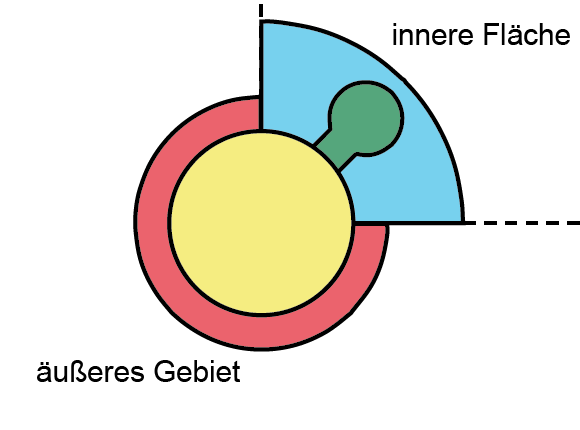
\includegraphics[height=150px]{Bilder/CornerPin2D-07.png}
\end{Bild}
Die Summe aller Objekte des Typs \icode{CornerPin} repräsentieren den untere Abschnitt des Eckpfeilers, welcher die Verbindungen der Grundplatten mit diesem gewährleistet.
Hierfür besteht ein einzelner Eckpin aus einem Zylinder, einer Ausstülpung seitens diesem und einem Zylindersegment.
Das Grundgerüst wird durch den Basiszylinder des Eckpfeilers festgelegt, welcher auch beim Eckzylinder vorkommt.
Für die Ausstülpung gilt, dass sie aus einem Quader mit angrenzendem Zylinder aufgebaut ist.
Die Länge des Quaders ist dabei abhängig von dem Winkel zwischen den beiden Wänden, welche die Grundplatte an dem Eckpfeiler begrenzen.
Er wird stets so lang berechnet, dass die Ausstülpung(siehe Abbildung, grün dargestellt) einen definierten Abstand von den Wänden einnimmt(siehe \ref{params}).
Für die untere Abgrenzung des Pinkopfes(siehe Abbildung \thebildnr, hellblau) berechnet die Anwendung eine Schnittmenge zwischen der angrenzenden Fläche und einem flachen Zylinder.\\
Falls ein Eckpin für das äußere Gebiet berechnet werden soll, wird anstatt der oben beschriebenen Elementen eine Differenzmenge zwischen der Umrandungsfläche des Grundrisses und dem flachen Zylinder gebildet.
Dies resultiert in ein Zylindersegment, wie es in Abbildung \thebildnr (rot) zu sehen ist.
Ein Eckpfeiler hat so einen stabilisierten unteren Abschnitt, auch außerhalb des Grundrisses.


\subsection{Wandstücke}
Eine Wand verkörpert eine Kante der DCEL.
Für die Erstellung dieser wird ein Quader mit der Länge der entsprechenden Kante gebildet und nach dieser rotiert.
Jeweils ein Eckzylinder wird anschließend an den Start- bzw. Endknoten des Quaders verschoben, sodass zwischen diesem und den beiden Eckzylindern eine Differenzmenge gebildet werden kann.
Das Resultat ist eine Wand, welche abschließend in einen Eckpfeiler eingesetzt werden kann. 
\begin{Bild}{Querschnitt einer Wand}
	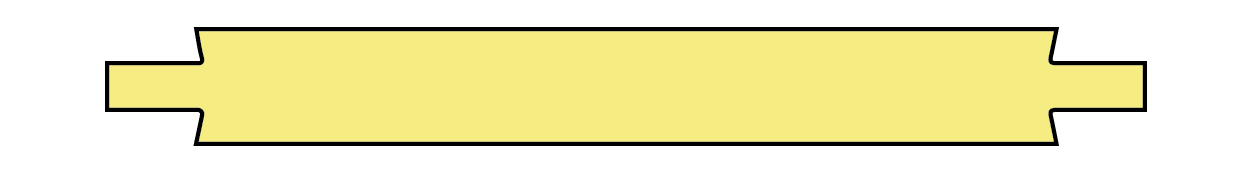
\includegraphics[width = 110mm]{Bilder/Wand2D-04}
\end{Bild}
\begin{Bild}{Ein Wand in der OpenSCAD Darstellung (Screenshot der Verfasser)}
	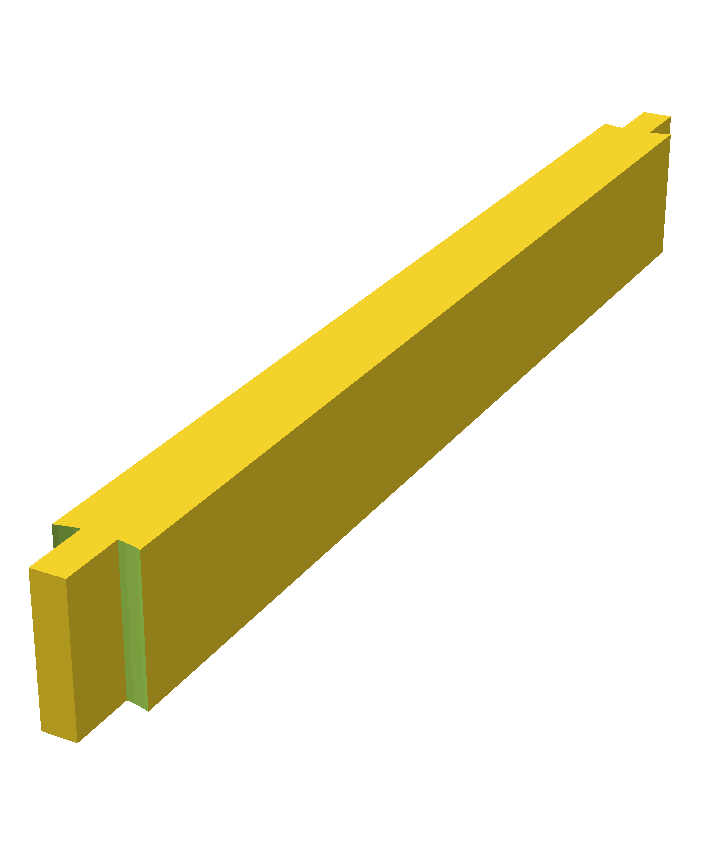
\includegraphics[height=200px, width=240px]{Bilder/Untereinheit_Wand}
\end{Bild}



\subsection{Grundplatten}
Eine Grundplatte wird anhand einer Fläche des Grundrisses konstruiert.
Sie sind aufgebaut aus einem geradem Prisma mit einer Polygon-Grundfläche, welches eingestülpte Steckmechanismen an der Unterseite besitzt.
\begin{Bild}{Stecker einer Grundplatte}
	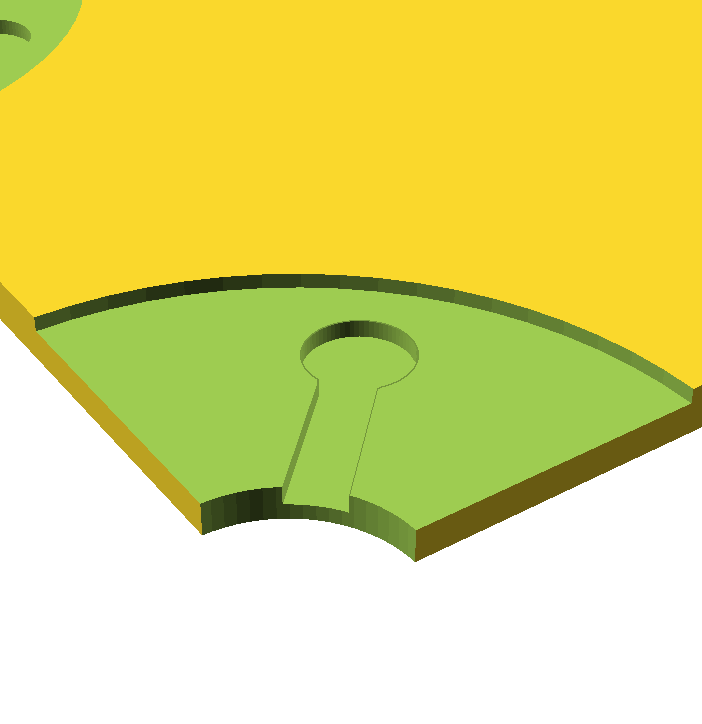
\includegraphics[height=200px]{Bilder/Untereinheit_GP}
\end{Bild}
Für die Berechnung des 3D-Objekts, wird an jedem Knoten der Fläche wird ein Eckpin gebildet und von dem polygonalen Prisma abgezogen, sodass genannte Einkerbungen durch eine Differenzmenge entstehen. 
Jede Grundplatte, die an das äußere Gebiet angrenzt wird zudem an dieser Seite um die halbe Wanddicke vergrößert, damit ein abgeschlossener Eindruck des gesamten 3D-Modells entsteht.(Siehe Abbildung \thebildnr)
\begin{Bild}{Vergrößerung der äußeren Grundplatten(vereinfacht)}
	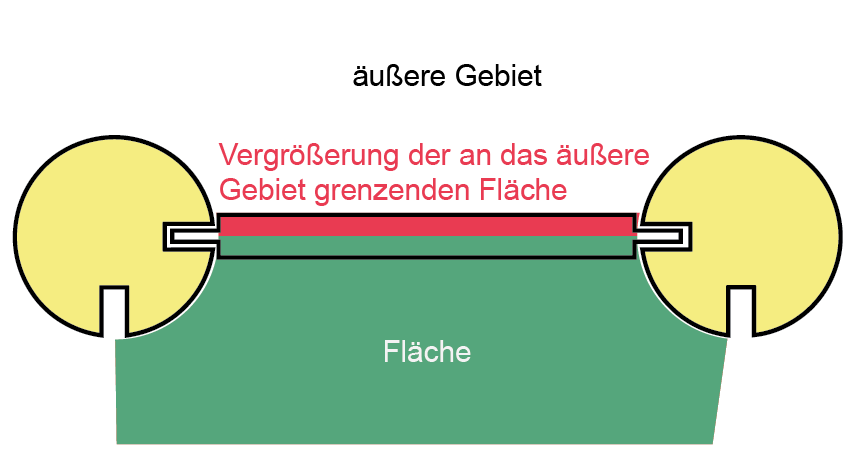
\includegraphics[width=120mm]{Bilder/GrundplatteVergroesserung-08}
\end{Bild}

\subsection{Zuweisen von Berechnungskonstanten}
\label{params}
Die \icode{Params}-Klasse dient als Speichermöglichkeit für alle nötigen Konstanten, welche für die Umrechnung des Grundrisses in das 3D-Modell benötigt werden.
Jedem dreidimensionalen Objekt benötigt eine Instanz einer solchen Klasse, um den OpenSCAD Code zu generieren.
In der Anwendung wird von der Klasse \icode{ScadProcessor} die angegebenen Parameter an alle Elemente des Grundrisses weitergegeben, damit verhindert wird, dass unterschiedliche Komponenten desselben Grundrisses verschiedene Konstanten zur Verfügung gestellt bekommen.
Sie werden bei Beginn des Programms in der \icode{Main}-Klasse gesetzt und können über eine Instanz der \icode{Params}-Klasse aufgerufen werden.

\begin{code} [Die \icode{setParams()}-Funktion zum Setzen der Parameter]
	public void setParams(double E, ...){
		e = E;
		// ...
	}
\end{code}

Das Abrufen der Parameter erfolgt dann mittels der entsprechenden \icode{get()}-Funktionen der \icode{Params}-Klasse, welche für alle Parameter vorhanden sind.
Der Aufbau der \icode{get()}-Funktionen folgt dem generellen Aufbau des nachfolgenden Codebeispiels, jedoch werden die Parameterbezeichnungen jeweils entsprechend ersetzt:\\

\begin{code} [Die \icode{get()}-Funktion für den Parameter \icode{e}]
public double getE() {
	return e;
}
\end{code}

Die nötigen Parameter stellen dabei Gleitkommazahlen(\icode{double}) dar, die verschiedene Teile des Grundrisses beeinflussen. 
Theoretisch können sie alle variiert werden.

\subsubsection{$\epsilon$/Epsilon}
Der Parameter Epsilon($\epsilon$) bezeichnet einen Abstand zwischen 3D-Objekten, der benötigt wird, um einem möglichen Fehler des 3D-Druckers entgegenzuwirken.
Dieser kann z.B. bewirken, dass Steckmechanismen nicht ineinander passen.
Deswegen tritt der Abstand $\epsilon$ generell dort auf, wo zwei Objekte aufeinander oder ineinander geschoben werden müssen.
In Folgenden Teilen des 3D-Modells tritt Epsilon auf:
\begin{compactenum}
	\item Bei dem Vorkommen von einem positven und einem negativem Steckern (Wand/Eckpfeiler und Grundplatte/Eckpfeiler) ist der negative gleichmäßig um$\epsilon$ vergrößert, damit ein abschließendes Stecken ermöglicht wird.
	\item Wenn zwei Grundplatten aufeinandertreffen, wird die sich berührenden Seiten um $0.5*\epsilon$ entgegengesetzt zueinander verschoben zur Einhaltung eines Abstandes von $\epsilon$ 
	\item Die Höhe einer Wand wird um $\epsilon$ verringert, damit die Oberseite des gesamten 3D-Objekts eine glatte Oberfläche besitzt.
\end{compactenum}

Das im Programm definierte Epsilon wurde mittels einem Experiment(siehe Abbildung \thebildnr) ermittelt.
Dafür wurde ein Stecker und Einstülpungen, die um ein verschiedenes $\epsilon$ vergrößert wurden, gedruckt, sodass getestet wurden konnte, welches Epsilon für den MakerBot Replicator\texttrademark\ 2 am geeignetsten ist.
Ausgewertet wurde daraus ein Wert von 0.25mm.
So erkennt man, dass dieser Parameter druckerspezifisch.
\begin{Bild}{Versuch zur Ermittlung eines passenden Epsilon-Wertes}
		\includegraphics[width=120mm]{Bilder/EpsilonTest_cut-09}
\end{Bild}

\begin{description}[style=nextline]
	\item[E ($\epsilon$/Epsilon)] 
		Der Parameter \q{E} entspricht der Konstante $\epsilon$ (Epsilon), welcher aus Gründen der vorteilhaften Kürze der Parameternamen hier verwendet wurde.
		Somit muss nicht jedes mal \icode{Epsilon} ausgeschrieben werden, es wird auf \icode{E} reduziert.
		$\epsilon$ bezeichnet den Abstand, welcher zwischen zwei Bauteilen mit einberechnet werden muss, um ein einfaches Zusammenstecken zu gewährleisten.
	\item[CornerRadius]
		Der Parameter \q{CornerRadius} entspricht der Konstante, welche den Radius des Grundzylinders der Eckstücken angibt.
	\item[PinMinLength] 
		Der Parameter \q{PinMinLength} entspricht der Konstante, welche die minimale Länge des Quaders des positiven Eckstücks angibt, welcher zwischen dem Eckzylinder und dem Pinzylinder platziert wird.
	\item[PinPWidth] 
		Der Parameter \q{PinPWidth} entspricht der Konstante, welche die Weite für den Quader des positiven Eckstücks angibt, welcher zwischen dem Eckzylinder und dem Pinzylinder platziert wird.
	\item[PinPRadius] 
		Der Parameter \q{PinPRadius} entspricht der Konstante, welche den Radius des Pinzylinders des positiven Eckstücks angibt.
	\item[PinDistance]
		Der Parameter \q{PinDistance} entspricht der Konstante, welche die Distanz zwischen dem positiven Pin und den anliegenden Wandstücken angibt, welche für jeden Pin eingehalten werden muss.
	\item[Height]
		Der Parameter \q{Height} entspricht der Konstante, welche die Höhe der Wandteile und der Eckzylinder angibt.
	\item[PinHeight]
		Der Parameter \q{PinHeight} entspricht der Konstante, welche die Höhe des positiven Pinzylinders angibt.
	\item[BasePlateHeight]
		Der Parameter \q{BasePlateHeight} entspricht der Konstante, welche die Höhe der Grundplatte angibt.
	\item[BasePlatePinCircleHeight]
		Der Parameter \q{BasePlateCircleHeight} entspricht der Konstante, welche die Höhe der Kreisflächen angibt, die unter den positiven Eckstücken angebracht werden und der Stabilisierung und Verankerung von Grundplatter und Eckstück dienen.
\end{description}